

%% Allow footnotes in longtable head/foot
%\IfFileExists{footnotehyper.sty}{\usepackage{footnotehyper}}{\usepackage{footnote}}
%\makesavenoteenv{longtable}
%\usepackage{graphicx}
%\makeatletter
%\newsavebox\pandoc@box
%\newcommand*\pandocbounded[1]{% scales image to fit in text height/width
%  \sbox\pandoc@box{#1}%
%  \Gscale@div\@tempa{\textheight}{\dimexpr\ht\pandoc@box+\dp\pandoc@box\relax}%
%  \Gscale@div\@tempb{\linewidth}{\wd\pandoc@box}%
%  \ifdim\@tempb\p@<\@tempa\p@\let\@tempa\@tempb\fi% select the smaller of both
%  \ifdim\@tempa\p@<\p@\scalebox{\@tempa}{\usebox\pandoc@box}%
%  \else\usebox{\pandoc@box}%
%  \fi%
%}
%% Set default figure placement to htbp
%\def\fps@figure{htbp}
%\makeatother
%\setlength{\emergencystretch}{3em} % prevent overfull lines
%\providecommand{\tightlist}{%
%  \setlength{\itemsep}{0pt}\setlength{\parskip}{0pt}}
%\usepackage{bookmark}
%\IfFileExists{xurl.sty}{\usepackage{xurl}}{} % add URL line breaks if available
%\urlstyle{same}
%\hypersetup{
%  hidelinks,
%  pdfcreator={LaTeX via pandoc}}
%
%\author{}
%\date{}
%
%\begin{document}

This section confronts one of the most formidable challenges in the
evolution of blockchain technology: scalability. As decentralized
networks gain mainstream adoption, their ability to process a high
volume of transactions in a timely and cost-effective manner becomes
paramount. We will begin by exploring the conceptual framework of the
``blockchain trilemma,'' a term coined by Vitalik Buterin, which posits
that it is inherently difficult to simultaneously optimize for
scalability, security, and decentralization.

We will then embark on a comprehensive survey of the various approaches
that have been proposed to address this challenge. Our exploration will
encompass both Layer 1 and Layer 2 scaling solutions. At Layer 1, we
will examine protocol-level enhancements such as Bitcoin-NG, which
decouples leader election from transaction processing, and sharding, a
technique that partitions the network into smaller, more manageable
units. We will also explore the potential of Directed Acyclic Graph
(DAG) based protocols as an alternative to the traditional linear
blockchain structure.

Furthermore, we will consider the role of permissioned blockchains and
Trusted Execution Environments (TEEs) in achieving scalability,
acknowledging the trade-offs they entail in terms of decentralization.
By the end of this section, you will have a nuanced understanding of the
complex and multifaceted challenge of blockchain scalability and the
diverse range of solutions that are being developed to address it.

\subsection{Learning Objectives}\label{learning-objectives}

\begin{itemize}
\tightlist
\item
  Understand the concept of blockchain scalability and the blockchain
  trilemma.
\item
  Learn about different metrics for evaluating blockchain performance,
  such as throughput, latency, and finality.
\item
  Explore naive approaches to improving scalability and their
  limitations.
\item
  Grasp the concept of Bitcoin-NG and how it decouples leader election
  from transaction serialization.
\item
  Understand the principles of sharding and how it can be used to
  parallelize transaction processing.
\item
  Learn about DAG-based protocols as an alternative to traditional
  blockchain structures.
\item
  Gain insight into the role of permissioned blockchains and Trusted
  Execution Environments (TEEs) in achieving scalability.
\end{itemize}

\begin{center}\rule{0.5\linewidth}{0.5pt}\end{center}

\subsection{The Scalability
Challenge}\label{section-1-the-scalability-challenge}

\subsubsection{Defining Scalability}\label{defining-scalability}

Scalability in the context of blockchain can be defined in two primary
ways:

\begin{enumerate}
\def\labelenumi{\arabic{enumi}.}
\tightlist
\item
  \textbf{Throughput:} This refers to the capability of the system to
  handle a growing amount of work, measured by the number of actions
  (transactions) processed in a given time frame. It is commonly
  expressed in \textbf{transactions per second (TPS)}.
\item
  \textbf{Number of Nodes:} This refers to the ability of the network to
  maintain its performance (e.g., TPS) as the number of participating
  nodes grows. A truly scalable system should not see its performance
  degrade as more nodes join the network.
\end{enumerate}

\subsubsection{The Blockchain
Trilemma}\label{the-blockchain-trilemma}

The blockchain trilemma is a conceptual model, popularized by Ethereum
co-founder Vitalik Buterin, that illustrates the inherent trade-offs in
designing a blockchain system (see \autoref{fig:trillema}). It posits that a blockchain can only
fully satisfy two of the following three properties at any given time:

\begin{itemize}
\tightlist
\item
  \textbf{Scalability}: The ability of the network to process a high
  volume of transactions (high TPS).
\item
  \textbf{Decentralization}: The ability of the network to run without
  any trust dependencies on a small group of centralized actors.
\item
  \textbf{Security}: The ability of the network to resist a large
  percentage of malicious participating nodes (e.g., 51\% for Bitcoin,
  33\% for BFT).
\end{itemize}

\begin{figure}[t]
	%	\vspace{-0.3cm}
	\begin{center}
		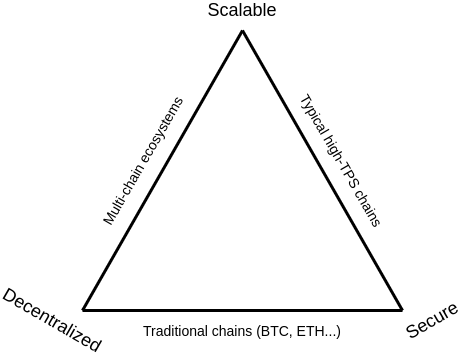
\includegraphics[width=0.6\textwidth]{./figs/trillema.png}
		\caption{The Blockchain
			Trilemma.}		
		\label{fig:trillema}
	\end{center}	
\end{figure}



This trilemma leads to different classes of solutions, each making a
specific trade-off:

\begin{itemize}
\tightlist
\item
  \textbf{A) Traditional L1 Chains (e.g., Bitcoin, Ethereum 1.0):}
  Prioritize decentralization and security, sacrificing scalability.
\item
  \textbf{B) High-TPS Chains (e.g., BFT-based):} Prioritize scalability
  and security, sacrificing decentralization.
\item
  \textbf{C) Multi-chain Ecosystems (e.g., Sharding, L2s):} Prioritize
  scalability and decentralization, but can have lower security as an
  attacker only needs to compromise a single shard.
\end{itemize}

\subsubsection{Throughput Limitations in
Practice}\label{throughput-limitations-in-practice}

The difference in throughput between traditional blockchains and
centralized systems is stark, highlighting the need for scaling
solutions (see \autoref{tab:throu}).

\begin{table}
\centering


\begin{tabular}{ll}

	\toprule
	\textbf{System} & \textbf{Throughput (TPS)} \\
	\midrule
	Bitcoin & 3 - 8  \\
	Ethereum & 15 - 30 \\
	Solana & 5,000  (lab tested) \\
	VISA & 11,000 - 25,000  \\
	\bottomrule
\end{tabular}
	\caption{Throughput of various blockchains vs. VISA.}\label{tab:throu}
	
\end{table}


\subsubsection{The Blockchain Stacked
Model}\label{the-blockchain-stacked-model}

Scalability can be addressed at different layers of the blockchain
stack~\cite{homoliak2020security}:


\begin{itemize}
\tightlist
\item
  \textbf{Network Layer:} Propagating transactions efficiently.
\item
  \textbf{Consensus Layer:} Ordering transactions efficiently.
\item
  \textbf{RSM (Replicated State Machine) Layer:} Executing smart
  contracts and interpreting transactions.
\item
  \textbf{Application Layer:} Interactions between contracts and chains.
\end{itemize}

\begin{center}\rule{0.5\linewidth}{0.5pt}\end{center}

\subsection{Forks, Finality, and
Metrics}\label{section-2-forks-finality-and-metrics}

\begin{table}[b]
	
	\begin{center}
		\begin{tabular}{ll}
			\toprule
			System & Finality Time \\
			\midrule
			Bitcoin & \textasciitilde60 min (6 blocks) \\
			Ethereum PoW & \textasciitilde3 min (12 blocks) \\
			Ethereum PoS & \textasciitilde12 min (2 epochs) \\
			Algorand & Instant \\
			\bottomrule
			
		\end{tabular}
	\end{center}
	\caption{Finality of various blockchains.}\label{tab:finality}
	
\end{table}


\subsubsection{Forks in PoW
Blockchains}\label{forks-in-pow-blockchains}

Forks occur when two or more miners find a block at roughly the same
time, creating temporary branches in the chain. This leads to ``stale''
or ``orphaned'' blocks that are eventually discarded.

%\begin{figure}
%\centering
%%\pandocbounded{\includegraphics[keepaspectratio,alt={Fork illustration}]{../../../Input/BDA-09-Scalability-Throughut-10.-4.-2025_files/Image_012.jpg}}
%\caption{Fork illustration}
%\end{figure}

Forks create the risk of \textbf{double-spending}, where a value spent
in one branch is spent again in another. This is why transaction
confirmation requires waiting for a certain number of blocks to be added
after the transaction's block, a concept known as \textbf{finality}.

\subsubsection{Finality}\label{finality}

Finality is the time it takes for a transaction to be considered
irreversible. Different systems have vastly different finality times (see \autoref{tab:finality}).



\subsubsection{Blockchain Metrics}\label{blockchain-metrics}

Several metrics are used to evaluate the performance and scalability of
a blockchain:

\begin{itemize}
\tightlist
\item
  \textbf{Throughput (TPS):} How many transactions can be processed per
  second.
\item
  \textbf{Latency:} The time it takes to propagate a transaction across
  the entire network.
\item
  \textbf{Finality:} The time it takes for a transaction to become
  irreversible.
\item
  \textbf{Stale Block Rate:} The percentage of mined blocks that are
  orphaned.
\item
  \textbf{Fairness:} The proportion of rewards relative to the invested
  mining power.
\end{itemize}

\begin{center}\rule{0.5\linewidth}{0.5pt}\end{center}

\subsection{Layer 1 Scaling
Solutions}\label{section-3-layer-1-scaling-solutions}

Layer 1 scaling solutions involve making fundamental changes to the core
protocol of the blockchain.

\subsubsection{Naive Improvements and Their
Limitations}\label{naive-improvements-and-their-limitations}

The most intuitive approaches to improving scalability involve simply
adjusting the protocol's parameters, but these have significant
drawbacks.

\begin{itemize}
\item
  \textbf{Increasing the Block Size:} While this allows more
  transactions per block, larger blocks take longer to propagate,
  leading to a higher stale block rate and favoring miners with better
  network connections, thus increasing centralization.

%  \begin{figure}
%  \centering
%%  \pandocbounded{\includegraphics[keepaspectratio,alt={Increased Block Size Problem}]{../../../Input/BDA-09-Scalability-Throughut-10.-4.-2025_files/Image_024.png}}
%  \caption{Increased Block Size Problem}
%  \end{figure}
\item
  \textbf{Decreasing the Block Creation Time:} This also increases the
  theoretical TPS but leads to more frequent forks and a higher stale
  block rate, which wastes resources and weakens security.

%  \begin{figure}
%  \centering
%%  \pandocbounded{\includegraphics[keepaspectratio,alt={Decreased Block Time Problem}]{../../../Input/BDA-09-Scalability-Throughut-10.-4.-2025_files/Image_029.png}}
%  \caption{Decreased Block Time Problem}
%  \end{figure}
\end{itemize}

%As shown in the graph below, decreasing the block creation time dramatically increases the orphan block rate.

%\begin{figure}
%\centering
%%\pandocbounded{\includegraphics[keepaspectratio,alt={Orphan Block Rate vs.~Block Time}]{../../../Input/BDA-09-Scalability-Throughut-10.-4.-2025_files/Image_030.png}}
%\caption{Orphan Block Rate vs.~Block Time}
%\end{figure}

\subsubsection{Bitcoin-NG (Next
Generation)}\label{bitcoin-ng-next-generation}

Bitcoin-NG~\cite{eyal2016bitcoinNG} is a more sophisticated Layer 1 scaling solution that
improves throughput by decoupling leader election from transaction
serialization.

\textbf{Principle:} 1. \textbf{Leader Election (Key Blocks):} A leader
is elected via Proof-of-Work, creating a ``key block.'' This block does
not contain transactions but secures the leader's right to publish
transactions. 2. \textbf{Transaction Serialization (Microblocks):} The
elected leader then serially publishes transactions in smaller
``microblocks'' without needing to perform PoW for each one (see \autoref{fig:bitcoin-ng}). This
continues until a new leader mines a new key block.

%\begin{figure}
%\centering
%%\pandocbounded{\includegraphics[keepaspectratio,alt={Bitcoin-NG Principle}]{../../../Input/BDA-09-Scalability-Throughut-10.-4.-2025_files/Image_035.jpg}}
%\caption{Bitcoin-NG Principle}
%\end{figure}

This approach allows for much higher transaction throughput, as it is
limited only by the network's propagation capacity and the leader's
processing power, not by the PoW mining interval. However, it introduces
a new vulnerability: the leader becomes a single point of failure and a
target for Denial-of-Service (DoS) attacks. 
Bitcoin-NG shows significantly better scalability
than Bitcoin, although it does not achieve perfect linear scaling.
The transaction fees are split across the current and the next leader in ratio 40\% vs. 60\% to incetivize the next miner on continuing of the most recent chain of blocks (see \autoref{fig:bitcoin-ng2}).



\begin{figure}[t]
	%	\vspace{-0.3cm}
	\begin{center}
		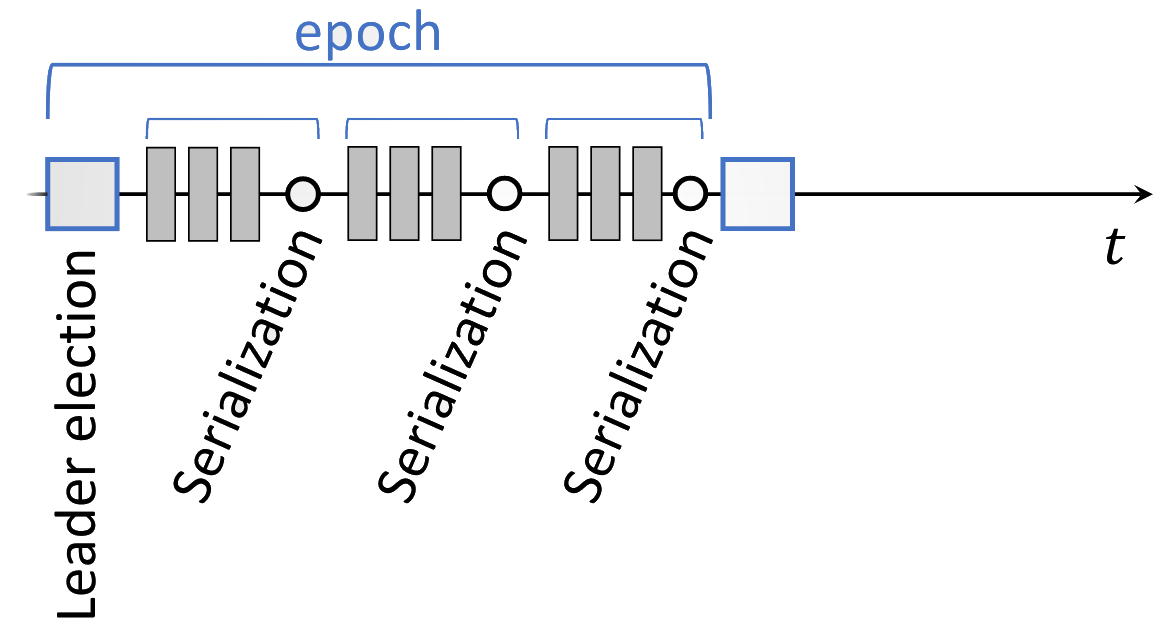
\includegraphics[width=0.6\textwidth]{./figs/bitcoin-ng.png}
		\caption{Bitcoin-NG principle.}		
		\label{fig:bitcoin-ng}
	\end{center}	
\end{figure}

%\begin{figure}
%\centering
%%\pandocbounded{\includegraphics[keepaspectratio,alt={Bitcoin-NG Evaluation}]{../../../Input/BDA-09-Scalability-Throughut-10.-4.-2025_files/Image_041.jpg}}
%\caption{Bitcoin-NG Evaluation}
%\end{figure}

\begin{figure}[b]
	%	\vspace{-0.3cm}
	\begin{center}
		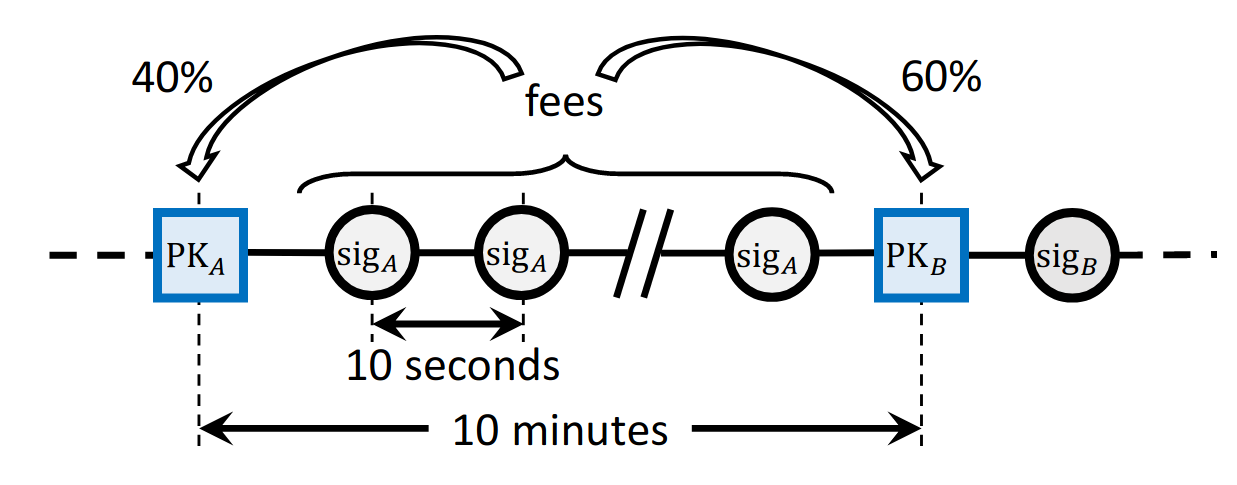
\includegraphics[width=0.7\textwidth]{./figs/bitcoin-ng2.png}
		\caption{Bitcoin-NG: split of transaction fees.}		
		\label{fig:bitcoin-ng2}
	\end{center}	
\end{figure}




\subsubsection{Sharding}\label{sharding}

Sharding is a powerful technique for scaling blockchains that is
borrowed from the world of distributed databases. It involves
partitioning the state of the blockchain (accounts, transactions, etc.)
into smaller, more manageable pieces called \textbf{shards}. Each shard
is then processed by a different subset of nodes (a committee) in the
network (see also \autoref{fig:sharding}). This allows for parallel transaction processing, which can lead
to a linear increase in throughput as the number of nodes in the network
grows.

%\begin{figure}
%\centering
%%\pandocbounded{\includegraphics[keepaspectratio,alt={Horizontal Sharding}]{../../../Input/BDA-09-Scalability-Throughut-10.-4.-2025_files/Image_046.jpg}}
%\caption{Horizontal Sharding}
%\end{figure}

\begin{figure}[t]
	%	\vspace{-0.3cm}
	\begin{center}
		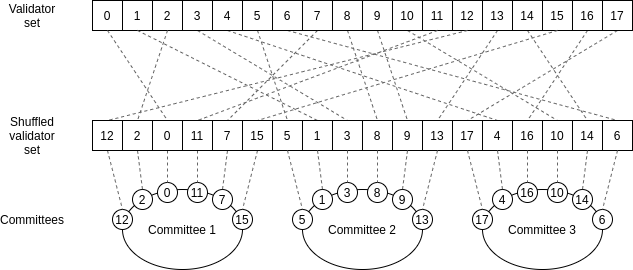
\includegraphics[width=0.7\textwidth]{./figs/sharding.png}
		\caption{Sharding: splitting the validators into committees.}		
		\label{fig:sharding}
	\end{center}	
\end{figure}


\paragraph{Elastico.}\label{elastico}
Elastico~\cite{luu2016secure} was the first practical sharding protocol proposed for open
blockchains.
%
\textbf{Design:} 1. \textbf{Identity Establishment:} Nodes perform a PoW
task. The resulting hash determines their identity and committee
assignment. 2. \textbf{Committee Formation:} Nodes are divided into
smaller committees (shards) based on their PoW solution. A final
``directory committee'' is also formed to finalize blocks. 3.
\textbf{Intra-Committee Consensus:} Each committee processes a subset of
transactions and reaches consensus using a BFT-like protocol. 4.
\textbf{Final Consensus:} The directory committee collects the processed
blocks from each shard and broadcasts a final, unified block to the
network (see also \autoref{fig:elastico}).

\begin{figure}[b]
	%	\vspace{-0.3cm}
	\begin{center}
		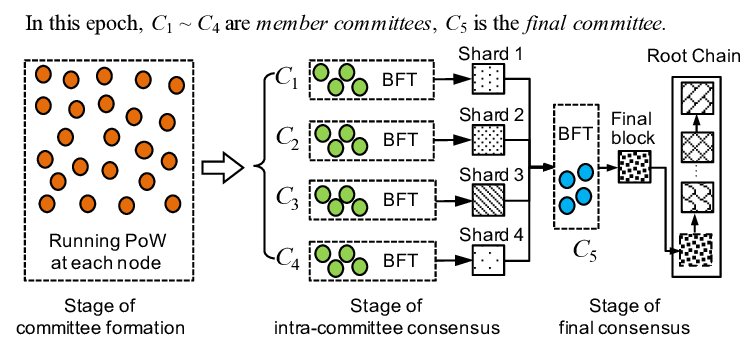
\includegraphics[width=0.7\textwidth]{./figs/elastico.png}
		\caption{Elastico stages of committee formation.}		
		\label{fig:elastico}
	\end{center}	
\end{figure}


\textbf{Evaluation:} Elastico demonstrated that throughput could scale
nearly linearly with the number of nodes. However, a significant amount
of time was spent on committee formation, and it lacked a mechanism for
secure cross-shard transactions.

%\begin{figure}
%\centering
%%\pandocbounded{\includegraphics[keepaspectratio,alt={Elastico Evaluation}]{../../../Input/BDA-09-Scalability-Throughut-10.-4.-2025_files/Image_073.png}}
%\caption{Elastico Evaluation}
%\end{figure}

\paragraph{OmniLedger.}\label{omniledger}

OmniLedger~\cite{kokoris2018omniledger} builds upon Elastico with several key improvements.
\textbf{Design Goals:}  \textbf{Security:} Full decentralization, shard
robustness, and secure cross-shard transactions.  \textbf{Performance:}
Scale-out, low storage, and low latency.

\textbf{Key Innovations:} \textbf{RandHound:} A secure and unbiased
randomness protocol used for validator assignment to shards, preventing
adversarial manipulation. \textbf{Atomix:} A protocol for secure,
atomic cross-shard transactions. It ensures that transactions spanning
multiple shards either commit atomically or abort completely.
\textbf{ByzCoinX:} A robust and efficient intra-shard BFT consensus
protocol.

%\begin{figure}
%\centering
%%\pandocbounded{\includegraphics[keepaspectratio,alt={OmniLedger Architecture}]{../../../Input/BDA-09-Scalability-Throughut-10.-4.-2025_files/Image_080.png}}
%\caption{OmniLedger Architecture}
%\end{figure}

\textbf{Evaluation:} OmniLedger demonstrated significant performance
gains over previous systems, achieving high throughput with low latency.

%\begin{figure}
%\centering
%%\pandocbounded{\includegraphics[keepaspectratio,alt={OmniLedger Throughput}]{../../../Input/BDA-09-Scalability-Throughut-10.-4.-2025_files/Image_087.jpg}}
%\caption{OmniLedger Throughput}
%\end{figure}

\paragraph{RapidChain.}\label{rapidchain}

RapidChain~\cite{zamani2018rapidchain} aims for \textbf{full sharding}, partitioning not only
computation but also storage and communication. This approach promises
even greater scalability by minimizing redundancy across the network.

%\begin{figure}
%\centering
%%\pandocbounded{\includegraphics[keepaspectratio,alt={RapidChain Comparison}]{../../../Input/BDA-09-Scalability-Throughut-10.-4.-2025_files/Image_093.png}}
%\caption{RapidChain Comparison}
%\end{figure}

\subsubsection{DAG-Based Protocols}\label{dag-based-protocols}

Directed Acyclic Graph (DAG) based protocols represent a fundamental
departure from the linear chain structure of traditional blockchains. In
a DAG-based system, each block refers one or more previous
blocks, creating a graph-like structure. This allows for parallel
transaction processing and can result in significantly higher throughput
and lower confirmation times (see example in \autoref{fig:dag}).

%\begin{figure}
%\centering
%%\pandocbounded{\includegraphics[keepaspectratio,alt={PHANTOM DAG}]{../../../Input/BDA-09-Scalability-Throughut-10.-4.-2025_files/Image_100.png}}
%\caption{PHANTOM DAG}
%\end{figure}

\begin{figure}[t]
	%	\vspace{-0.3cm}
	\begin{center}
		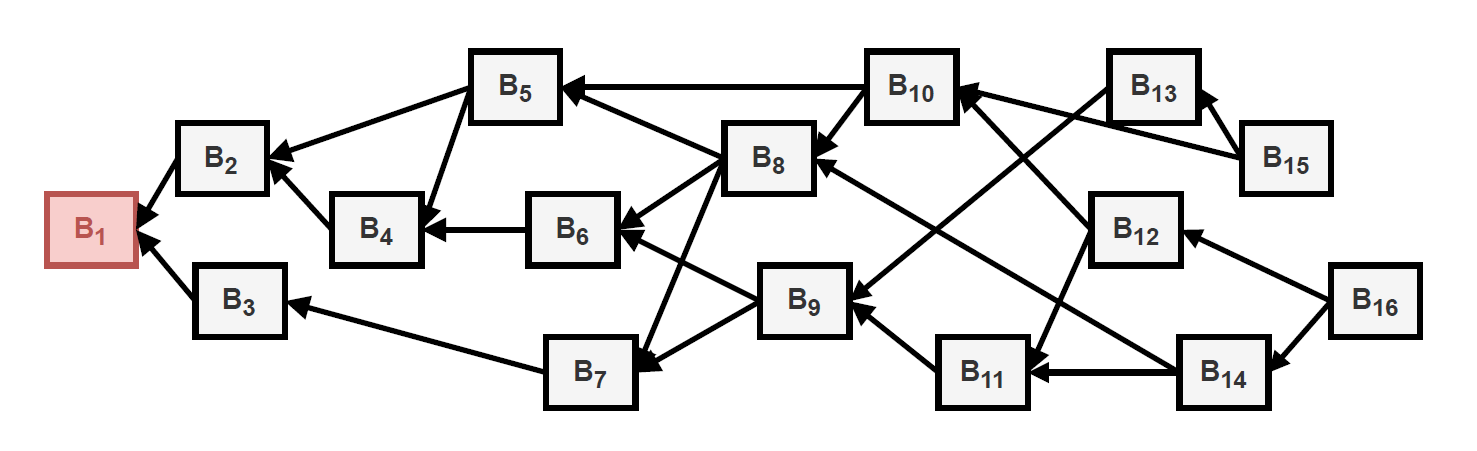
\includegraphics[width=0.7\textwidth]{./figs/DAG.png}
		\caption{Example of DAG-based structure of the blockchain.}		
		\label{fig:dag}
	\end{center}	
\end{figure}

However, DAGs introduce new challenges, such as achieving a total
ordering of transactions, which is an NP-hard problem. Protocols like
 \textbf{PHANTOM} and its optimization \textbf{GHOSTDAG}~\cite{sompolinsky2020phantom}  have been developed to address these challenges, but they remain an active area of research.
Phantom is a generalization of Nakamoto’s PoW longest chain protocol that utilized DAGs instead of a single chain. 
The complexity of recursively determining the order of the blocks it contains is impractical for efficient use and requires solving an NP-hard problem (the maximal k-cluster SubDAG problem). Therefore, a greedy algorithm called GHOSTDAG has been developed.
The key idea of this protocol is that it performs a complete ordering of all blocks (transactions) and includes orphaned blocks, except an attacker-created blocks that are weakly connected.
The general problem of such DAG-based designs is that they rely on random transation selection to avoid duplicates across blocks. 
However, a greedy rational attacker might ignore such an altruistic choice and select transactions based the highest fees to maximize their profit~\cite{perevsini2023incentive,perevsini2021dag}.
This has an adversarial effect on the effective throughput of the network, having much more transaction duplicates across different blocks.


\begin{figure}[t]
	%	\vspace{-0.3cm}
	\begin{center}
		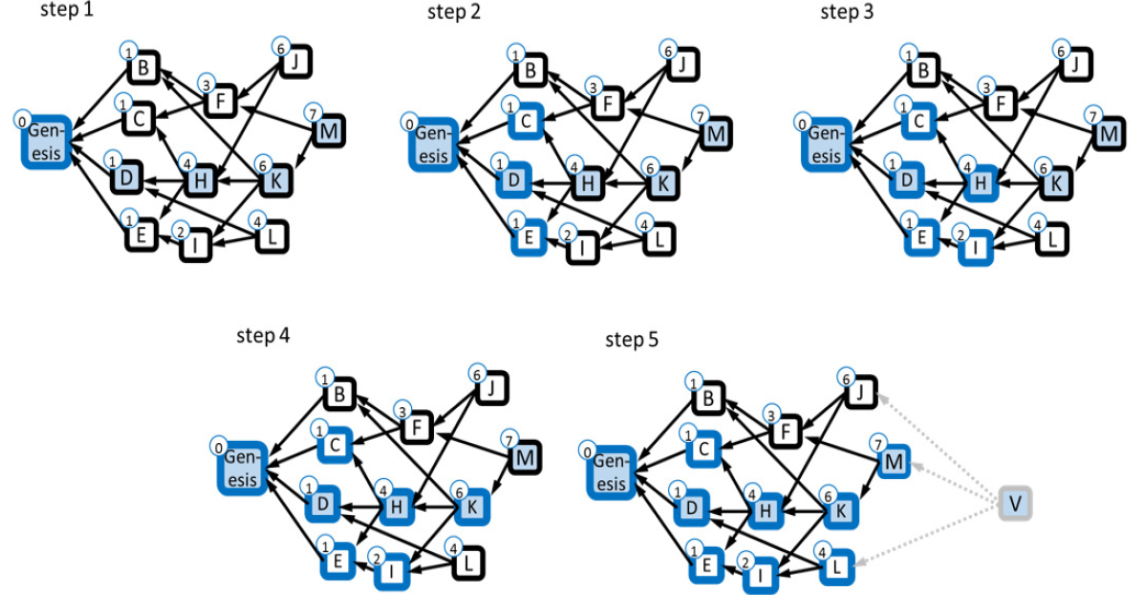
\includegraphics[width=0.8\textwidth]{./figs/PHANTOM.png}
		\caption{Ordering of blocks in PHANTOM and elimination of weakly connected blocks.}		
		\label{fig:phantom}
	\end{center}	
\end{figure}
 

\paragraph{Sycomore.}\label{sycomore}
Sycomore~\cite{anceaume2018sycomore} is a DAG-based protocol that features a self-adapting
structure and defends against the incentive attack mentioned above. 
In particular Sycomore mandates each transaction to be included only in a specific chain, based on the prefix of the transaction hash.
The DAG can split into more parallel chains when transaction
demand is high and merge back together when demand is low, dynamically
adjusting the level of parallelism (see \autoref{fig:sycomore}).



\begin{figure}[t]
	%	\vspace{-0.3cm}
	\begin{center}
		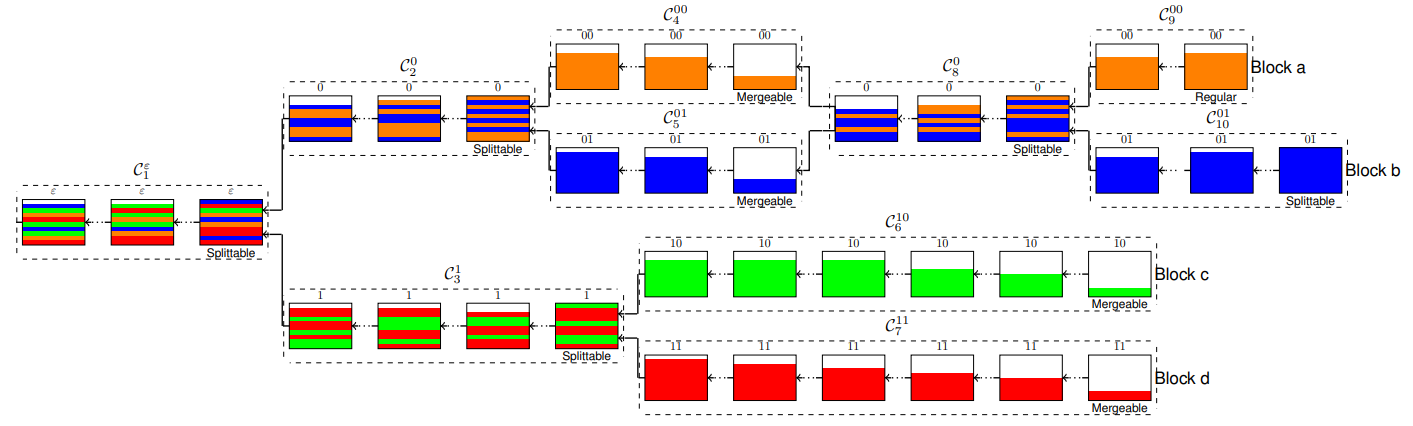
\includegraphics[width=0.9\textwidth]{./figs/Sycomore.png}
		\caption{Sycomore -- splitting and mergin the chains based on the demand.}		
		\label{fig:sycomore}
	\end{center}	
\end{figure}




%\begin{figure}
%\centering
%%\pandocbounded{\includegraphics[keepaspectratio,alt={Sycomore Self-Adaptivity}]{../../../Input/BDA-09-Scalability-Throughut-10.-4.-2025_files/Image_106.jpg}}
%\caption{Sycomore Self-Adaptivity}
%\end{figure}

\begin{center}\rule{0.5\linewidth}{0.5pt}\end{center}

\subsection{Layer 2 and Other Scaling
Solutions}\label{section-4-layer-2-and-other-scaling-solutions}

\subsubsection{Layer 2 Scaling}\label{layer-2-scaling}

Layer 2 solutions operate on top of an existing Layer 1 blockchain,
handling transactions off-chain to reduce the load on the main chain.

\begin{itemize}
\item
  \textbf{Payment Channels (e.g., used in Bitcoin Lightning~\cite{poon2016bitcoin}):} Users open a
  channel by locking funds on the main chain. They can then conduct
  numerous transactions off-chain within that channel, only settling the
  final balance on the main chain when the channel is closed.
  If multiple such channels are combined into a single network, any two indirectly interconnected users can transact through intermediaries, who obtain a certain routing fee (see also \autoref{section-5-the-lightning-network-a-scalability-solution}).

%  \begin{figure}
%  \centering
%%  \pandocbounded{\includegraphics[keepaspectratio,alt={Layer 2 Payment Channels}]{../../../Input/BDA-09-Scalability-Throughut-10.-4.-2025_files/Image_107.png}}
%  \caption{Layer 2 Payment Channels}
%  \end{figure}
\item
  \textbf{ZK-Rollups:} Transactions are processed off-chain, and a
  cryptographic proof (a ZK-SNARK) is generated to attest to their
  validity. This single proof is then submitted to the Layer 1 chain,
  allowing a large batch of transactions to be verified with a single
  on-chain transaction.
\end{itemize}

\subsubsection{Permissioned
Blockchains}\label{permissioned-blockchains}

Permissioned blockchains offer a different approach to scalability by
restricting network access to a known set of participants. This allows
for the use of more efficient, non-PoW consensus mechanisms like
Byzantine Fault Tolerance (BFT).

\begin{itemize}
\tightlist
\item
  \textbf{Hyperledger Fabric and BESU:} A popular enterprise-grade framework that
  uses a modular architecture with components for ordering services,
  membership providers, and smart contract execution.
  However, a single point of failure of Hyperledger fabric is a centralized ordering service. 
  In contrast, Hyperledger BESU is using a variant of BFT, called IBFT, which has security properties of standard BFT consensus protocols.
  
  
\end{itemize}

\subsubsection{Trusted Execution Environments
(TEEs)}\label{trusted-execution-environments-tees}

A Trusted Execution Environment (TEE) is a secure and isolated area of a
main processor that provides confidentiality and integrity guarantees
for code and data. TEEs, such as \textbf{Intel SGX}, can be used to
create hybrid blockchain solutions that offload some of the
computational work from the main blockchain to a trusted hardware
environment, improving scalability and privacy.
Example of technologies are Intel SGX, ARM TrustZone, Keystone Enclave.
In this systems, even remote client can verify what code is running within the enclave -- this process is called remote attestation.
There have been many attacks on TEE platform in the past, such as VoltPillager~\cite{chen2021voltpillager} or Plundervolt~\cite{murdock2020plundervolt}.

There were proposed some blockchain and centralized ledgers~\cite{homoliak2020aquareum} that utilize TEE to increase the processing throughput and/or to provide privacy of transactions~\cite{cheng2019ekiden}.  

%\begin{figure}
%\centering
%%\pandocbounded{\includegraphics[keepaspectratio,alt={Intel SGX}]{../../../Input/BDA-09-Scalability-Throughut-10.-4.-2025_files/Image_119.png}}
%\caption{Intel SGX}
%\end{figure}

\begin{center}\rule{0.5\linewidth}{0.5pt}\end{center}

\subsection{Summary / Key Takeaways}\label{summary-key-takeaways}

This section has provided a comprehensive overview of the critical
challenge of blockchain scalability. We have established that there is
no single, perfect solution, but rather a spectrum of approaches that
involve different trade-offs between scalability, security, and
decentralization, as encapsulated by the blockchain trilemma.

We have explored a variety of Layer 1 scaling solutions, from naive
approaches like increasing the block size to more sophisticated
techniques like Bitcoin-NG, sharding, and DAG-based protocols. We have
also examined Layer 2 solutions like payment channels and ZK-Rollups, as
well as alternative architectures like permissioned blockchains and
TEEs.

The key takeaway is that the pursuit of scalability is an ongoing and
dynamic area of research. As the technology matures, we can expect to
see the emergence of new and innovative solutions that combine these
different approaches to push the boundaries of what is possible in terms
of performance, security, and decentralization.

\begin{center}\rule{0.5\linewidth}{0.5pt}\end{center}

\subsection{Keywords}\label{keywords}

\begin{itemize}
\tightlist
\item
  \textbf{Scalability}: The ability of a blockchain network to handle a
  growing number of transactions and users without compromising
  performance.
\item
  \textbf{Blockchain Trilemma}: The widely held belief that a blockchain
  system can only fully satisfy two of the following three properties:
  scalability, security, and decentralization.
\item
  \textbf{Throughput (TPS)}: The number of transactions that a
  blockchain network can process per second.
\item
  \textbf{Finality}: The time it takes for a transaction to be
  considered permanent and irreversible.
\item
  \textbf{Layer 1 Scaling}: Protocol-level changes that aim to improve
  the scalability of the blockchain itself.
\item
  \textbf{Bitcoin-NG}: A Layer 1 scaling solution that decouples leader
  election from transaction serialization.
\item
  \textbf{Sharding}: A technique for partitioning the state of a
  blockchain into smaller, more manageable pieces called shards.
\item
  \textbf{DAG (Directed Acyclic Graph)}: A data structure that allows
  for parallel transaction processing and can be used as an alternative
  to a linear blockchain.
\item
  \textbf{Layer 2 Scaling}: Solutions that operate on top of a Layer 1
  blockchain to improve scalability.
\item
  \textbf{Permissioned Blockchain}: A type of blockchain that restricts
  access to a limited set of participants.
\item
  \textbf{Trusted Execution Environment (TEE)}: A secure and isolated
  area of a main processor that can be used to offload computation from
  the main blockchain.
\end{itemize}

\begin{center}\rule{0.5\linewidth}{0.5pt}\end{center}

\subsection{Further Reading}\label{further-reading}

\begin{itemize}
\tightlist
\item
  \textbf{The Blockchain Trilemma}:\\
  \url{https://vitalik.ca/general/2021/04/07/sharding.html}
\item
  \textbf{Bitcoin-NG: A Scalable Blockchain Protocol}: \\
  \url{https://www.usenix.org/system/files/conference/nsdi16/nsdi16-paper-eyal.pdf}
\item
  \textbf{Elastico: A Secure Sharding Protocol for Open Blockchains}: \\
  \url{https://www.comp.nus.edu.sg/\textasciitilde loiluu/papers/elastico.pdf}
\item
  \textbf{OmniLedger: A Secure, Scale-Out, Decentralized Ledger}: \\
  \url{https://eprint.iacr.org/2017/406.pdf}
\item
  \textbf{RapidChain: A Secure, Fast and Scalable Blockchain}: \\
  \url{https://www.usenix.org/conference/usenixsecurity19/presentation/zamani}
\end{itemize}